% ANL Beamer template
\documentclass[aspectratio=169]{beamer}
\usepackage[english]{babel}
\usepackage[utf8]{inputenc}

% AMSLaTeX packages
\usepackage{amsthm}
\usepackage{amsmath}
\usepackage{amsfonts}
\usepackage[algoruled]{algorithm2e}

\usetheme{default}
\useoutertheme{default}
% we want to use images
\usepackage{graphicx}
\usepackage{movie15}
\usepackage{hyperref}

% table relates packages
\usepackage{booktabs}
\usepackage{multirow}
% pick a font
\usepackage{palatino}           
% \usepackage{times}
\usepackage{tikz}
\usetikzlibrary[positioning,arrows,decorations.pathmorphing,backgrounds,fit,calc]
% \AtBeginSection[]  % "Beamer, do the following at the start of every section"
% {
%   \begin{frame}<beamer> 
%     \frametitle{Outline} % make a frame titled "Outline"
%     \tableofcontents[currentsection]  % show TOC and highlight current section
%   \end{frame}                    
% }

% \AtBeginSubsection[]
% {
%   \begin{frame}
%     \frametitle{Outline}
%     \tableofcontents[currentsection,currentsubsection]
%   \end{frame}
% }

\AtBeginSection[]
{
   \begin{frame}
       \frametitle{Outline}
       \tableofcontents[currentsection]
   \end{frame}
}

\newcommand{\ebox}[1][1em]{\framebox[#1]{\phantom{M}}}

\setlength\arraycolsep{1.4pt}% some length

%gets rid of navigation symbols
\setbeamertemplate{navigation symbols}{}

%gets rid of bottom navigation bars
\setbeamertemplate{footline}[page number]{}
\setbeamertemplate{headline}{}


\usebackgroundtemplate{\includegraphics[width=\paperwidth]{../templates/NormalANLBlue}}

% Define big arrow down
\newcommand{\xdownarrow}[1]{%
  {\left\downarrow\vbox to #1{}\right.\kern-\nulldelimiterspace}
}

\usepackage{xcolor,ulem}

% Title/author info
\title{\bigskip
\\
ParMOO: A Python library for parallel multiobjective simulation optimization}
\author{Tyler Chang$^a$ and Stefan Wild$^{a,b}$}
\institute{$^a$Mathematics and Computer Science Division,\\
Argonne National Laboratory\\

\medskip

$^b$Applied Mathematics and Computational Research Division,\\
Lawrence Berkeley National Laboratory}
\date{SIAM CSE 23}

% Slides start here
\begin{document}

% Set the background graphics
\setbeamertemplate{footline}{}
{
\usebackgroundtemplate{\includegraphics[width=\paperwidth]{../templates/TitleANLBlue}}
\frame{\titlepage}
}
\setbeamertemplate{footline}[page number]{}

% FRAME: overview
\begin{frame}
  \frametitle{Outlines}
  \tableofcontents
\end{frame}

% ========================================
% main slides come here
% ========================================

\section{Introduction to MOOPs}

\begin{frame}\frametitle{Multiobjective Optimization Problems}
\begin{center}
\onslide<1->{
{\Large
$$
\min_{x \in \mathcal{X}} F(x)
$$
}}
\end{center}
\begin{columns}
\begin{column}{.35\textwidth}
\onslide<2->{
\includegraphics[width=\textwidth]{feasible_design.eps}
}
\end{column}
\begin{column}{.2\textwidth}
\begin{center}
\onslide<2->{
$\xrightarrow{\hspace*{2cm}}$
$$
F : {\cal X} \rightarrow {\cal Y}
$$
}
\onslide<3->{
expensive blackbox process
}
\end{center}
\end{column}
\begin{column}{.35\textwidth}
\onslide<2->{
\includegraphics[width=\textwidth]{convex_pareto.eps}
}
\end{column}
\end{columns}
\end{frame}

\begin{frame}\frametitle{Multiobjective Response Surface Methodology}
{or Model-Based Optimization or Active Learning}
\begin{columns}
\begin{column}{0.4\textwidth}
\begin{center}
\onslide<2->{
\includegraphics[width=0.6\textwidth]{lh_doe.eps}\\}
\medskip
\vskip 0.5cm
\medskip
\onslide<5->{
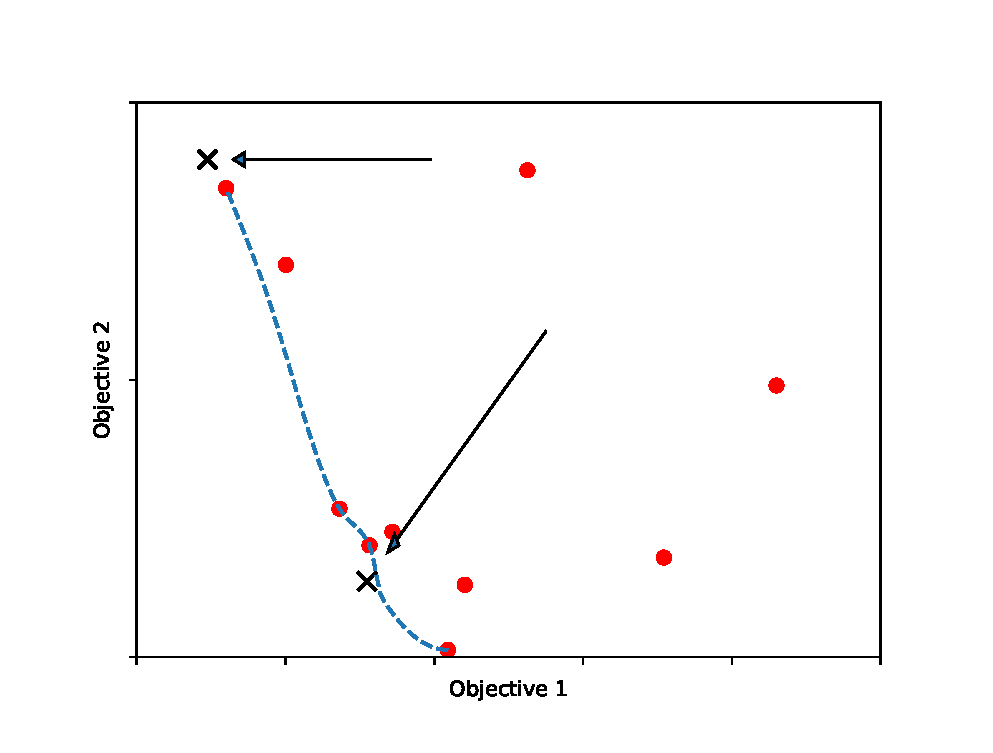
\includegraphics[width=0.6\textwidth]{tradeoff.eps}}
\end{center}
\end{column}
\begin{column}{0.2\textwidth}
\begin{center}
\onslide<3->{
$\xrightarrow{\hspace*{1.5cm}}$}\\
\vskip 1.2cm
\onslide<6->{
$\qquad\qquad\nearrow$\\
{\Huge $\mathcal{C}$}\\
$\nearrow\qquad\qquad$}\\
\vskip 1cm
\onslide<5->{
$\xleftarrow{\hspace*{1.5cm}}$}
\end{center}
\end{column}
\begin{column}{0.4\textwidth}
\begin{center}
\onslide<3->{
\includegraphics[width=0.58\textwidth]{lab_setup.jpg}}\\
\medskip
\onslide<4->{
$\xdownarrow{0.5cm}$\\
\medskip
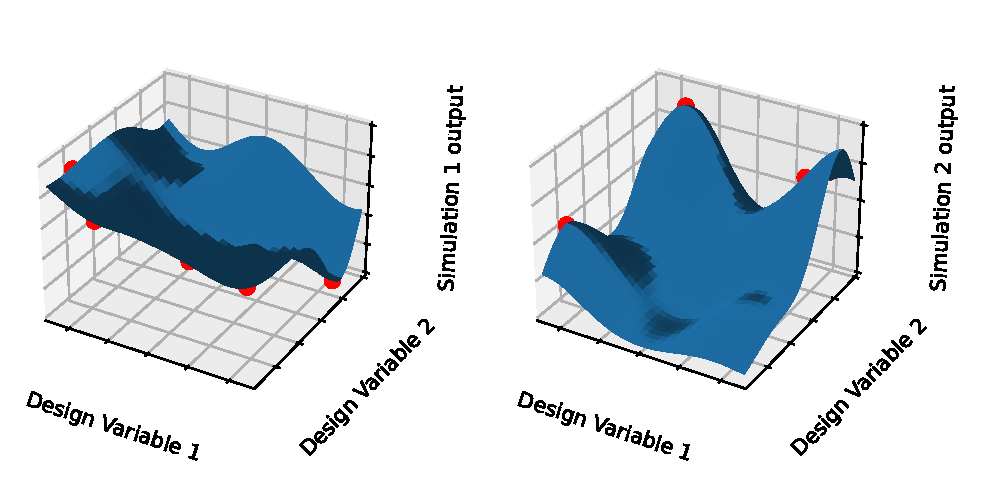
\includegraphics[width=0.9\textwidth]{rsm.eps}}
\end{center}
\end{column}
\end{columns}
\end{frame}

\begin{frame}\frametitle{Example: HPC library tuning}



\end{frame}

\section{ParMOO Design Criteria}

\begin{frame}\frametitle{ParMOO Design Criteria}

\textbf{Design goals:}
\begin{enumerate}
\item Highly customizable framework for multiobjective RSM
\item Exploit structure and domain knowledge simulation-based optimization
problems
\item Flexible problem types (mixed-variables, constraints, etc.)
\end{enumerate}

\medskip
\pause

\textbf{Design constraints:}
\begin{enumerate}
\item Easy to deploy (parallelism, checkpointing, logging, flexibility)
\item Easy to maintain and extend
\item Easy to use (clean interfaces)
\end{enumerate}
\end{frame}

\begin{frame}\frametitle{Customizability}
ParMOO uses an object-oriented framework:\\
\begin{columns}
\begin{column}{0.7\textwidth}
\includegraphics[width=\textwidth]{algorithm-flowchart.png}
\end{column}
\begin{column}{0.3\textwidth}
\pause
\begin{itemize}
\item Search/DOE
\item Surrogate model
\item Acquisition function
\item Single-obj solver
\end{itemize}
\end{column}
\end{columns}
\end{frame}

\begin{frame}\frametitle{Simulation Structure}
\begin{center}
\onslide<1>{
\includegraphics[height=2in]{des-obj-space.png}}

\vskip -2in

\onslide<2>{
\includegraphics[height=2in]{des-sim-obj-space.png}}
\end{center}
\end{frame}

\begin{frame}\frametitle{Simulation Structure}
\pause
{\Large
$$
f_i(x) = {\color{blue}h_i(x, {\color{red}S(x)} )}
\qquad i = 1, \ldots, o
$$
}
\begin{columns}
\begin{column}{0.5\textwidth}
\pause
\textbf{Sum-of-squares structure:}

\medskip

{\large
$$
{\color{blue} h_i(x, S(x)) = \sum_{j \in N_i} \big({\color{red}S_j(x)}\big)^2}
$$

where each ${\color{blue} N_1, \ldots, N_o}$ is an index set.
}

\bigskip

Increases order of approximation $\Rightarrow$
increases order of convergence

\end{column}
\begin{column}{0.5\textwidth}
\pause
\textbf{Heterogeneous MOOPs:}

{\large
\begin{align*}
{\color{red} h_1(x, S(x)) = S_1(x)}\\
{\color{blue} h_2(x, S(x)) = \|x \|^2}
\end{align*}
}

Use expensive surrogate models for {\color{red} $h_1$} (i.e.,
{\color{red} $S_1$}) but not for {\color{blue} $h_2$}

\end{column}
\end{columns}
\end{frame}

\begin{frame}\frametitle{Flexible Problem Types}
\begin{columns}
\begin{column}{0.8\textwidth}
\begin{itemize}
\onslide<2-> \item Mixed variable-types
\onslide<3->{ {\bf Ex: categorical variables}}
\begin{itemize}
\onslide<4-> \item Focus on {\it embedding} into continuous space\\
\bigskip
\bigskip

\end{itemize}
\onslide<5-> \item (Nonlinear) constraints
\begin{itemize}
\onslide<6-> \item Focus on {\it augmented Lagrangian} penalties
(relax to augmented unconstrained problem)
\end{itemize}
\end{itemize}
\end{column}
\begin{column}{0.2\textwidth}
\onslide<4->{
\includegraphics[width=0.95\textwidth]{embedder.png}}\\
\onslide<6->{
\includegraphics[width=1.2\textwidth]{feasible-region.png}}
\end{column}
\end{columns}
\end{frame}

\begin{frame}\frametitle{Design constraints}

\pause
{\bf Easy to use:}
\begin{itemize}
\item OOP gives a clean interface for adding attributes to a MOOP instance
\item Total modularity (free to mix-and-match)
%\pause \item Tried to balance flexibility vs. complexity
\end{itemize}

\bigskip
\pause
{\bf Easy to deploy:}
\begin{itemize}
%\pause \item Provides (optional) checkpointing, logging, and error handling
\item Simulation/experiment evaluations are only called in the
{\tt MOOP.solve()} method
\item Extend {\tt MOOP} class and overwrite {\tt solve()} to
deploy in different workflows
\item {\bf Ex:} Deploy parallel solvers on HPC systems using
{\tt libEnsemble}
\end{itemize}

\bigskip
\pause
{\bf Easy to maintain and extend:}
\begin{itemize}
\item OOP + total modularity makes adding new features easy
\item Agile development with continuous integration
\item Well-documented interface, contributing, and release process
\end{itemize}
\end{frame}

\section{Results and Sample Problems}

\begin{frame}\frametitle{ParMOO Release}

\begin{center}
\includegraphics[width=0.4\textwidth]{logo-parmoo.png}
\end{center}

\begin{columns}
\begin{column}{0.8\textwidth}

Written in {\tt Python} (available on {\tt pip} and {\tt GitHub})

\bigskip
\bigskip
\url{https://parmoo.readthedocs.io/en/latest/quickstart.html}

\bigskip
\bigskip
Combine with {\tt libEnsemble} to use parallel solvers
\end{column}
\begin{column}{0.2\textwidth}
\includegraphics[width=0.6\textwidth]{logo-py.png}

\bigskip

\includegraphics[width=0.4\textwidth]{logo-gh.png}
\end{column}
\end{columns}

\bigskip
\bigskip

{\small
Chang and Wild. 2022.
ParMOO: A Python library for parallel multiobjective simulation optimization.
Under review with JOSS.
}

\end{frame}

\begin{frame}\frametitle{Example 1: Fayans EDF Model Calibration}
Find params $x \in [0, 1]^{13}$ to fit the Fayans model to data $d_i$:
$$
M\left(\xi_{i};x\right) \approx d_{i} \qquad i=1,\ldots, 198
$$

\medskip

ParMOO simulation:
$$
S_{i}(x) = M\left(\xi_{i};x\right) - d_{i},
\qquad i=1,\ldots, 198;
$$

\medskip

\begin{columns}
\begin{column}{0.65\textwidth}
Min SOS across 3 observable classes
\end{column}
\begin{column}{0.35\textwidth}
$$
{\color{blue}F_t = \sum_{i=1}^{m_t}\big({\color{red}S_{t,i}(x)}\big)^2}
$$
\end{column}
\end{columns}

\vfill

{\small
Bollapragada et al. Journal of Physics G: Nuclear and Particle Physics 48(2), 2020.}\par
\end{frame}

\begin{frame}\frametitle{Fayans Solution with ParMOO}
\begin{columns}
\begin{column}{0.5\textwidth}
\begin{itemize}
\item Approximated Fayans model using inv dist weighting on existing dataset
\item {\color{blue}
Implemented parallel solver in ParMOO} using libEnsemble
\item Just {\bf 14-25 lines of Python code}
\item Ran for {\bf 10K} sim evals
\item Compared against
{\color{red} same solver w/o exploiting SOS structure}
\end{itemize}
\end{column}
\begin{column}{0.5\textwidth}
\includegraphics[width=\textwidth]{hv_1.eps}
\end{column}
\end{columns}
\end{frame}

\begin{frame}\frametitle{Example 2: Material Manufacturing with ParMOO}
Choose optimal settings for material manufacturing in a
continuous flow reactor (CFR)

\bigskip

We know how to make a desired material, need to produce at scale:

\begin{enumerate}
\item {\color{green} \bf Maximize the product} (battery electrolyte: TFML)
\item Can increase temperature to {\bf \color{red} reduce reaction time}
\item Too much heat activates a side reaction; need to
{\bf \color{blue} minimize unwanted byproduct}
\end{enumerate}

\bigskip
Challenges:

\begin{itemize}
\item Mixed variable types
\item Heterogeneous objectives
\item Must send experiments to run on CFR
\end{itemize}
\end{frame}

\begin{frame}\frametitle{CFR Optimization with ParMOO}

\begin{columns}
\begin{column}{0.5\textwidth}

\medskip
Extend {\tt MOOP} class to send/receive experiment data
using {\tt MDML} library (Apache Kafka)

\medskip
Used categorical variable embeddings

\medskip
Modeled Product/Byproduct as simulations and reaction time using algebraic
equation of input

\begin{center}
\includegraphics[width=0.5\textwidth]{lab_setup.jpg}\\
\end{center}
\end{column}
\begin{column}{0.5\textwidth}
\includegraphics[width=\textwidth]{pareto_front.png}
\end{column}
\end{columns}
\end{frame}

\begin{frame}\frametitle{Next Release}

Coming in v.~0.2
\begin{itemize}
\item Interactive post-run visualization tools
\item Support for customized embeddings and passing raw (unscaled) inputs
\item MDML (Apache Kafka) interface for distributing simulation evalutations
\item (Maybe) advanced techniques for design-of-experiments
\end{itemize}
\end{frame}

\begin{frame}\frametitle{Resources}
\begin{center}
{\large
E-mail: {\tt tchang@anl.gov}\\
E-mail: {\tt parmoo@mcs.anl.gov}\\
\bigskip
\bigskip
ParMOO is under review with JOSS\\
\bigskip
\bigskip
GitHub: {\tt github.com/parmoo/parmoo}\\
Docs: {\tt parmoo.readthedocs.io}\\
PyPI: {\tt pip install parmoo}}

\bigskip
\bigskip

{\small This material is based upon work supported by the U.S. Department of Energy, Office of Science, Office of Advanced Scientific Computing Research, SciDAC program under contract number DE-AC02-06CH11357.}
\end{center}
\end{frame}

\end{document}
